\chapter {\mbox{Cell/B.E.} programming}
\par
\mbox{Cell/B.E.} platform development tools will be described in this chapter.
Our experience with the tools will be mentioned as well.
Then particular SDK content and tools will be listed.
Parallel systems and models will be mentioned later on as well as the relationship to the \mbox{Cell/B.E.} development along with a few design patterns.
At the end core configurations and their advantages and disadvantages will be listed finishing with few practical approaches to the \mbox{Cell/B.E.} porting process.

\section{\mbox{Cell/B.E.} platform development}
\par
IBM delivers a SDK for the \mbox{Cell/B.E.} application development.
It is made for a Linux platform, in the concrete for the Fedora or the Red Hat distribution.
It comes in two flavours.
The first is the official non free SDK which has all the features needed for the \mbox{Cell/B.E.} development even for hybrid systems.
The purchaser has also a support team ready to help.
The next is a free one that is open to wide public and everybody can download it and start developing.
The free one does not have full support for hybrid systems nor for development in other languages than C/C++.
We have used the free one since we have developed only in C/C++ and for a clean \mbox{Cell/B.E.} processor.

\par
Because the SDK is for Linux operation system its user has to have already a deeper knowledge about this system.
There are a few bugs and parts that are not fully finished (see Appendix \ref{toolsSetup}) and without the deeper system knowledge is practically impossible to react on an unexpected behaviour during installation or development phase.

\par
We have begun with SDK version 3.0 and Fedora version 8 which were the current versions of needed tools.
We have faced a number of obstacles and before we were able to overcome them a new version of SDK (3.1) appeared.
Because we wanted to use and describe the latest tools we had to begin from scratch because the new version brought new obstacles as well.

\par
The new version was declared to be compatible with a new version of Fedora, 9 - Sulphur, that had been released at almost the same time as the new SDK version.
The previous version of SDK (3.0) was for Fedora 7 Werewolf.
We have tried all possible combinations of Fedora distributions and SDK packages to find out if they are compatible with each other.
The only result from that testings was finding out that they are not mutually compatible.
We have spent plenty of days on this discovery.
The SDK is a huge package of software dependent on lots of third party libraries and solutions.
They are treated differently within particular distributions and sometimes even versions of the same distribution.
The resulting advise is to avoid combination of system versions nor SDK versions nor particular libraries that the SDK components are dependent on.
The repository versions of the third party software should be used.

\par
Although there are too much of troubles when different version are combined, a few efforts to get the SDK run on another distributions than Fedora were made.
But we think the time spent on this goal is not worth the result.

\par
Finally we installed Fedora 9 Sulphur and SDK 3.1.
Although this combination is declared by IBM as tested we have run into few bugs and errors.
The process of installation is described in the Appendix \ref{toolsSetup}.

\section {SDK content}

The \mbox{Cell/B.E.} SDK is divided into variety of components.
Each component is contained in one or more rpm package for easy installation purposes.
Here is a list of important available components:
\begin{enumerate}
  \item {Tool chain}
  \par
  Is a set of tools such as compilers, linkers etc. necessary for actual code generation.
There are two tool chains.
One is for PPU and the other for SPU.

  \item {Libraries}
  \par
  IBM provides with the SDK several useful libraries for mathematical purposes e.g. linear algebra, FFT, Monte Carlo.
Another libraries set is for cryptography or run-time management.
Code of these libraries is debugged, highly optimized for running on SPEs and SIMDized.

  \item {Full system simulator}
  \par
  Program that can simulate the \mbox{Cell/B.E.} processor on other hardware platforms.
It is used mostly in profiling stage because simulator can simulate actual computation of a code in cycle precision.
It can be of course used when programmer has an actual \mbox{Cell/B.E.} hardware available, but the simulation is incredibly slow.

  \item {IDE}
  \par
  IDE is in fact version 3.2 of Eclipse with integration of debugging, profiling, \mbox{Cell/B.E.} machine management and other features that makes development for the \mbox{Cell/B.E.} easier and more comfortable.
\end{enumerate}


\section{Parallel systems \& \mbox{Cell/B.E.}}

Parallelism depends on type of system where the program will be run.
There are two basic kind of parallel systems:
\begin{enumerate}
\item {shared-memory system}
\par
Is a multi-processor system with one shared memory which all processor can see.
Processors has to synchronize access to the memory otherwise race conditions will rise.

\item {distributed-memory system}
\par
Is system where each processor has its own private memory.
There is no need for any synchronization.
\end{enumerate}

In context of parallel systems \mbox{Cell/B.E.} is a kind of hybrid system.
The SPEs matches a distributed-memory system due to private local stores while the PPE is a shared-memory system.
The \mbox{Cell/B.E.} is sometimes called heterogeneous multi-core processor with distributed memory.
Because \mbox{Cell/B.E.} processors can be composed into bigger units such as IBM blade server with two \mbox{Cell/B.E.} chips they can be viewed as either \mbox{16 + 2} cores in SMP mode or two non-uniform memory access machines connected together.
Programmer has then to decide which view of the \mbox{Cell/B.E.} processor is better for the solved problem.

\par
Because of separation of address spaces programming of the SPE is very similar to client/server application design.
Roles depends on how the work is started.
In case the PPU initiates the transfers, the PPU is a client and the SPE is a server because the SPE receive data for computation and offer a service for the PPE.
Another possibility is that the SPE grabs the data from the central memory.
In this case the SPE is a client of central memory.
This scenario is preferred because the PPE is only one and would not be able to manage all the SPUs.

\section{\mbox{Cell/B.E.} programming models}

\par
Implementation of parallel algorithms rely on a parallel programming model.
It is a set of software technologies such as programming languages extension, special compilers, libraries through that actual parallelism is achieved.
The programming model is programmer's view to the hardware.
Choosing a programming model or mixture of models that will best fit for the solved problem is another decision that programmer has to make.

\par
For the \mbox{Cell/B.E.} there is variety of parallel programming models.
THe models differ in view of the hardware from each other and thus how many actions are performed implicitly by the model.
The actions can be e.g. task distribution management, data distribution management or synchronization.
The most abstract ones can perform many actions implicitly.
Their advantage is ease of implementation but at cost no performance tuning ability.
Differently act the most concrete models that see the \mbox{Cell/B.E.} processor with all the low level details.
Their advantage is performance tuning ability in all application parts but at cost of more development.

\par
There are several models that are targeted only for the \mbox{Cell/B.E.} platform and are contained in the SDK.
While there are other models such as MPI, OpenMP that can be used as well but they would expose only the PPE.
These will not be further described.

List of the programming models (frameworks) follows in order from the most concrete to the most abstract:
\begin{enumerate}
\item {libspe2}
\par
This library provides the most low level functionality.
It offers SPE context creating, running, scheduling or deleting.
DMA primitives for data transfer, mailboxes, signal, events, and synchronization functions for PPE to SPE and SPE to SPE dialogues are also provided by this library.
More information can be found in \cite{performanceToolRef} within "SPE Runtime Management Library" document.

\item {Data Communication and Synchronization - DaCS}
\par
Defines a program entity for the PPE or the SPE.
It is a HE (Host Element program) for the PPE and an AE (Accelerator Element program) for the SPE.
It provides variety of services for that programs.
The services are e.g. resource and process management where an HE manipulates its AEs or group management, for defining groups in which synchronization events like barriers can happen or message passing by using send and receive primitives.
More information can be found in \cite{performanceToolRef} within "DACS Programmer's Guide and API Reference" document.

\item {Accelerated Library Framework - ALF}
\par
The ALF defines an ALF-task as another entity that perform computationally intensive parts of a program.
The idea is to have a program split into multiple independent pieces which are called work blocks.
They are described by a computational kernel, the input and the output data.
Programming with the ALF is divided into two sides.
The host and the accelerator one.
On the accelerator side the programmer has only to code the computational kernel, unwrap the input data, and pack the output data when the kernel finishes.
The ALF offers clear separation between host and accelerator sides of program parts.
It provides following services: work blocks queue management, load balancing between accelerators, transparent DMA transfers etc.
More information can be found in \cite{performanceToolRef} within "ALF Programmer's Guide and API Reference" document.

\end{enumerate}

Choosing a framework is important decision of writing \mbox{Cell/B.E.} application.
It should be considered enough.

\subsection {\mbox{Cell/B.E.} parallelism levels}

The \mbox{Cell/B.E.} processor offers four levels of parallel processing.
That is because it is composed of heterogeneous elements, the SPE and the PPE and the possibility of composition into a more complex systems.
The levels are:
\begin{enumerate}
\item Server level
\par
Parallelism on this level means task distribution among multiple servers like within a server farm.
This is possible in a hybrid environment at the cluster level using MPI or some other grid computing middle-ware.

\item \mbox{Cell/B.E.} chips level
\par
On this level tasks can be divided among multiple \mbox{Cell/B.E.} processors.
This is possible if there are more such processors in single machine.
It is e.g. IBM Blade server with two \mbox{Cell/B.E.} chips.
ALF or DaCS for hybrid can be used for task distribution.

\item SPE level
\par
This parallelism level allows to distribute tasks among particular SPEs.
Libspe, ALF, DaCS can be used to perform the distribution.

\item SIMD instruction level
\par
This level can increase the speed the most.
Parallelism is achieved on instruction level that means more data are processed at a time by single instruction.
Language intrinsics are used for this purpose.
This will be explained later in part devoted to "SIMDation".
\end{enumerate}

\subsection{Computation configurations}

\par
Because of the \mbox{Cell/B.E.}'s heterogeneous nature there are few computation configurations that can be used.
Each of them differs in usage of SPEs:
\begin{enumerate}
\item Streaming configuration
\par
All SPEs serves as a stream processor (see figure \ref{fg:streamingModel}).
They run exactly the same code expecting the same type of data and producing also the same of data type.
This configuration is well suited for streaming application for example filters where there is still the same type of data on input.

\begin{figure}
    \centering
    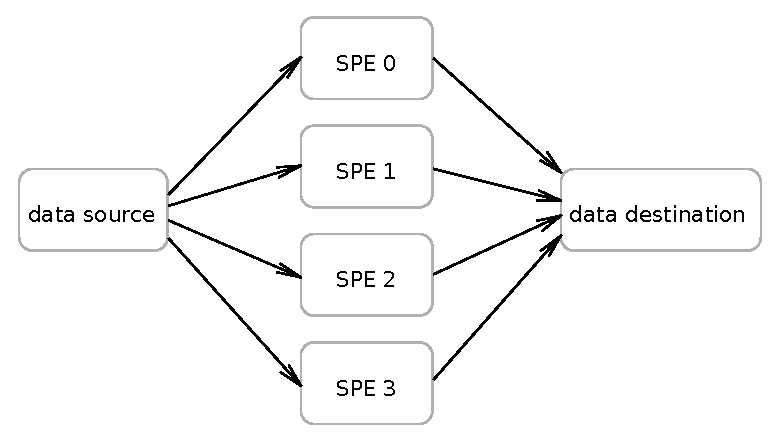
\includegraphics[width=0.9\textwidth]{data/streamingModel}
    \caption[Streaming SPE configuration]{All SPE run the same code creating farm of processor that process same type of data.}
    \label{fg:streamingModel}
\end{figure}

\item Pipeline configuration
\par
The SPEs are stages of a pipeline (see figure \ref{fg:pipelineModel}).
Data are passed through one SPE to another.
This configuration makes use of the fact that transfer among SPEs is faster than the transfer between SPE and PPE.

\begin{figure}
    \centering
    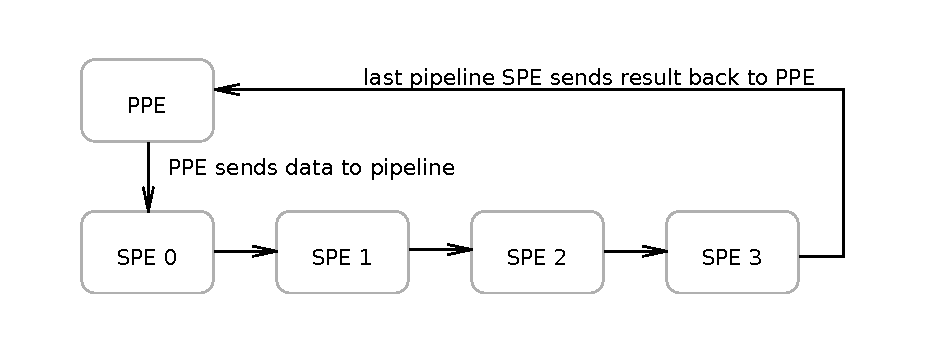
\includegraphics[width=0.9\textwidth]{data/pipelineModel}
    \caption[Pipeline SPE configuration]{SPE creates a pipeline. Each SPE represent one stage of that pipeline. Data are transferred only via SPE to SPE DMA transfers benefiting the speed of bus.}
    \label{fg:pipelineModel}
\end{figure}

\item PPE centric
\par
This configuration is common approach to use the \mbox{Cell/B.E.}
A program runs on the PPE (see figure \ref{fg:PPUCentricModel}) and only selected, highly computational intensive parts (hotspots) are offloaded to SPEs.
This method is the easiest from a program development perspective because it limits the scope of source code changes and does not require much re-engineering at the application logic level.
A disadvantage is frequent changes of SPE contexts that is quite expensive operation.

\begin{figure}
    \centering
    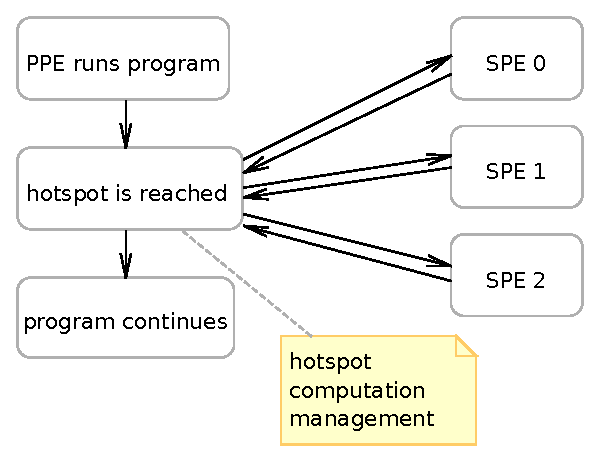
\includegraphics[width=0.7\textwidth]{data/PPUCentricModel}
    \caption[PPE centric configuration]{Program is run on PPE and only hotspots are offloaded to SPEs.
 Offloading means managing SPE context creation and loading as well as managing data transfer and synchronization between PPE and SPEs}
    \label{fg:PPUCentricModel}
\end{figure}

\item SPE server
\par
Another configuration is to have server-like programs running on SPEs that sits and waits offering specific services.
It is very similar to the PPE centric configuration.
Only difference is requirement to the program to be small enough to fit into the SPU local store to avoid the frequent SPE context switching.

\end{enumerate}

\section {Building for the \mbox{Cell/B.E.}}
\par
Actual compilation process is performed using an appropriate tool chain.
The PPE code requires the PPE tool chain and the SPE code requires the SPE one.
But there is a difference between management of the code in linking stage between the PPE and the SPE object files.
It is caused by difference of actual code usage.
While the PPU code resides in the central memory, like in common architectures, the SPU code is loaded into the SPE dynamically and shall be somehow separated from the PPE code.
It is similar to shader programs for graphic accelerators.
They are also loaded into appropriate processors as soon as they are needed so they live separated.

\par
There are two options for SPE code management.
One is to build a shared library and load it explicitly when it shall be used.
Another way is to build a static library and include it into the PPU executable using \mbox{Cell/B.E.} Embedded SPE Object Format (CESOF).
This allows PPE executable objects to contain SPE executable i.e. the SPE binary is embedded within the PPE binary, see figure \ref{fg:SPEEmbedding}.
The SPU program is then referenced as special external structure directly from the PPU code instead of performing shared library loading.
Both ways have advantages and disadvantages which are the same as shared vs. static library usage.
Shared library means better modularity and possibility of code alternation without whole executable rebuilding.
On the other hand additional management of such library is necessary in contrast to a static SPE code into a PPE binary embedding.


\begin{figure}
    \centering
    
\includegraphics[width=0.8\textwidth]{data/SPEEmbedding}
    \caption[SPE binary embedding]{Illustration how is a SPE binary "embedded" into a PPE binary.
The SPE binary is another section of the PPE binary.
It is reachable through extern struct variable, that contains a pointer to the SPE binary.}
    \label{fg:SPEEmbedding}
\end{figure}



\subsection {Process of application porting for the \mbox{Cell/B.E.}}
\label{sect:portingProcess}

Common process of application porting for the \mbox{Cell/B.E.} processor (figure \ref{fg:appPorting}) consists of next two basic steps:
\begin{enumerate}
\item Hotspots localization
\par
Through profiling of the application on the PPE we find most compute intensive parts, hotspots.
How to profile the application see chapter 5 of \cite{programmersGuide}.

\item Hotspot porting for SPE
\par
Each hotspot computation is moved to the SPE i.e. the code adaptation for the SPE features shall be performed.
This means DMA transfers instead of direct memory access, appropriate data structures utilization, etc.
Data movement tuning e.g. different data structures usage can be then performed until satisfactory performance is obtained.

\par
Work distribution among available SPEs shall be performed to accelerate actual computation.
Amount of work performed by particular SPEs should be equal to avoid mutual SPE waiting.
\end{enumerate}

\par
Following additional steps are necessary for application optimization and speed-up.
Performing these steps leads to utilization of all the SPU features such as whole register set utilization, dual-issuing of instructions, SIMD execution and DMA transfers.
More detail in \cite{writingPerfApps}, part 4:

\begin{enumerate}
\item{Multi-buffering}
\par
Data that resides within central memory and are processed by the SPE should be copied into local store before actual computation.
When there are more of the places for the data (buffers) the program can take advantage from asynchronous DMA transfer and can process current buffer while the next data are being transferred into another buffer.
Then the buffers are simply swapped and the SPU need not to wait until the transfer of next data is complete.
See the figure in the paragraph named "Hiding data-access latencies" in \cite{compilerOptions} for illustration.

\item{Branch elimination}
\par
Branch less instruction chain is a succession of instructions without any conditional jump.
In other words there is no decision where to continue performed within such succession.
Elimination of branches elongates the branch less instruction chain.
In such a chain all data always go through the same instructions which makes possible to perform SIMDation.
There is variety of branch elimination methods.
Good information resource provides \cite{cellPerformance}.
Branch elimination is probably the most complicated step due to necessity of complete code restructuralization.

\item{SIMDation}
\par
Means rewriting a scalar code into a vectorized one to be able to use SIMD instructions.
In this step the most performance gain could be achieved because of multiple data processing by one instruction.
Every single piece of data should go through the exactly same order of instructions in SIMDized code.
Therefore is necessary to have long branch less instruction chain.
The most important method is arrays of structure to structure of arrays conversion.
The figure in the paragraph called "SIMDizing" in \cite{compilerOptions} shall illustrate the data processing with SIMD instructions.

\par
SIMDizing brings also avoidance of usage a rotation instructions which are necessary to move unaligned data into preferred slot.
Preferred slot is the beginning of a register e.g. for short integer it is the first 16 bits of the register.

\item{Loop unrolling}
\par
Loop body is the code inside curly brackets of the loop.
This code is executed repeatedly until the loop condition is valid.
Loop unrolling means putting more loop bodies serially into the code.
This decrease loop count and elongate the loop body letting the compiler to make more optimizations.
Example:
\begin{verbatim}
for(uint32 i=0; i<32; i++)
{
    printf(".");
}
\end{verbatim}
become (by loop unrolling with factor 2)
\begin{verbatim}
for(uint32 i=0; i<16; i++)
{
    printf(".");
    printf(".");
}
\end{verbatim}
The compiler can do more optimizations e.g. better instruction scheduling and register utilization.

\item{Instruction scheduling}
\par
Proper reorganization of instructions can give more performance in some cases.
This step is performed by the compiler but it is possible to rearrange instructions manually in assembly language.

\item{Branch hinting}
\par
Gives a hint where the program is rather going to continue after future branch to the processor.
It is done through insertion of special instructions.
This step should be again accomplished by the compiler but it is possible to use appropriate assembly language instruction directly within the code.
\end{enumerate}

\begin{figure}
    \centering
    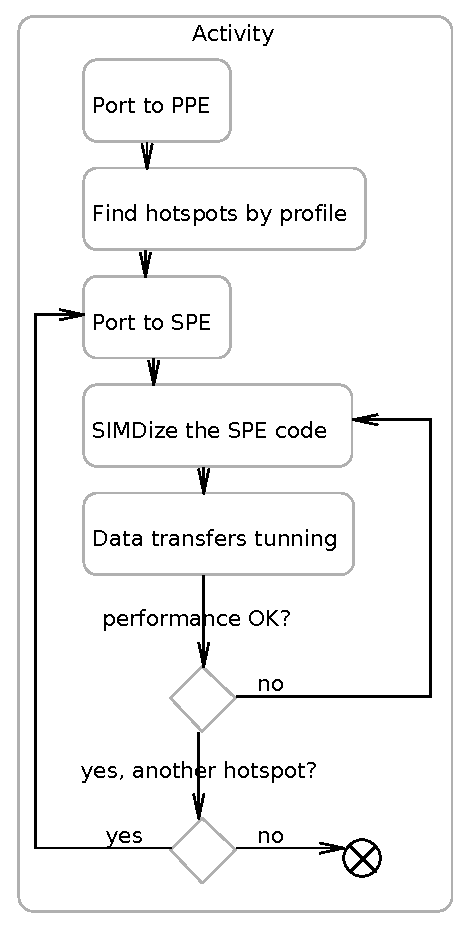
\includegraphics[width=0.5\textwidth]{data/portingCycle}
    \caption[Application porting cycle]{Diagram shows all stages of the process and loops for better performance tuning and other hotspots}
    \label{fg:appPorting}
\end{figure}

\subsection {SPE porting considerations}

\par
The local store size is the main SPE feature that everything spins around while porting a code to the SPE.
On the one hand there are decisions about data transfers.
This means how the data that has to be processed by the SPE will be transferred into local store and vice versa.
How many buffers will be used in case of multi-buffering.
On the other hand is code complexity of the solved problem that influence the size of the final binary.
There is one solution how to use bigger binaries than the local store, SPE overlays.
It is based on division of the binary into segments that are loaded into the SPE on demand in run-time.

\par
Programmer has to take into consideration all these things to make the final binary smaller than the local store.
Everything is big trade-off between the processed data chunk sizes, number of buffers for that chunks and the code lenght.

\par
After the first compilation of a SPU binary from original ported code the final executable will probably exceed the local store size even when the code does not seem as large.
Then a big searching what part of code causes the huge size would begin.
We have gone through several problems with code that is common in non SPE code but cause problems in the SPE code.
Here is the list:
\begin{enumerate}
\item usage of keyword new
\par
There is no memory allocation in the SPE. 
So usage of the \emph{new} keyword is meaningless.
But the SPE compiler accepts it without any complain.

\item usage of std streams
\par
This code:
\begin{verbatim}
#include <iostream>
std::cout << "Hello" << std::endl;
\end{verbatim}
goes through the compiler without complaints but makes the final binary very big.

\par
The reason why the resulting code is too big is probably size of the code within headers that are included when using described features.

\end{enumerate}

\subsection {Speed and compiler options}

\par
There is variety of compiler options.
Usage of them is worth nothing but can increase performance and avoid some kind of bugs.

\par
Mike Acton explains strict aliasing in \cite{strictAliasing}.
One advantage of usage of this feature is positive impact on performance.
Another advantage is fact that it can avoid bugs that would appear as far as in release stage when optimizations flags are used during compilation.
In this stage is really hard to track and debug this kind of bugs.

\par
Another option advises are in \cite{compilerOptions}

\section{Profiling}

\par
Profiling of \mbox{Cell/B.E.} application means rather profiling the SPE part of the application.
There is variety of profiling tools.
The basic one is a dynamic performance analysis which can provide many useful information such as how much time SPE stalled, reasons of the stall, the CPI (cycle per instruction) ratio, branch count, etc.
The next one is a static performance analysis which can illustrate run of a SPE in instruction precision.
These two analysis are evaluated from program run within full system simulator.
Both the methods are well described in tutorial in the cell IDE help which is accessible through menu $\rightarrow$ Help $\rightarrow$ Help Content in the IDE.

\par
Another profiling tools are:
\begin{enumerate}
\item{PDT - performance debugging tool}
\item{OProfile}
\item{CPC - cell performance counter}
\end{enumerate}

These tools collect profiling data that can be further processed with VPA (visual performance analyser), an external tool provided by IBM.
This tool can display the collected data in different charts, time lines or can highlight parts of the code that are worth to improve and many other useful features.
Usage of all these performance tools is described in SDK document "Performance Tools Reference" in \cite{performanceToolRef}.
We wanted to test them all but when we followed the manual instructions we experienced a few obstacles because we worked on PS3.
Lately, we have found out on forums that unfortunately there is poor or none support for these performance tools on PS3.
